%%%%
%% main.tex
%%
%% Copyright 2010 Jeffrey Finkelstein
%%
%% Except where otherwise noted, this work is made available under the terms of
%% the Creative Commons Attribution-ShareAlike 3.0 license,
%% http://creativecommons.org/licenses/by-sa/3.0/.
%%
%% You are free:
%%    * to Share — to copy, distribute and transmit the work
%%    * to Remix — to adapt the work
%% Under the following conditions:
%%    * Attribution — You must attribute the work in the manner specified by
%%    the author or licensor (but not in any way that suggests that they
%%    endorse you or your use of the work).
%%    * Share Alike — If you alter, transform, or build upon this work, you may
%%    distribute the resulting work only under the same, similar or a 
%%    compatible license.
%%    * For any reuse or distribution, you must make clear to others the 
%%    license terms of this work. The best way to do this is with a link to the
%%    web page http://creativecommons.org/licenses/by-sa/3.0/.
%%    * Any of the above conditions can be waived if you get permission from
%%    the copyright holder.
%%    * Nothing in this license impairs or restricts the author's moral rights.
%%%%
\documentclass[draft]{article}

% package imports
\usepackage[noend,linesnumbered,boxed]{algorithm2e} % for creating pseudocode
\usepackage{amsmath} % for piecewise function definition
\usepackage{amsthm} % for theorems, definitions, lemmas, and styles
\usepackage{amssymb} % for strict subset symbol (\subsetneq)
\usepackage{chngcntr} % for counting figures with section numbers
\usepackage{complexity} % for typesetting complexity classes
\usepackage{cclicenses} % for adding creative commons license symbols
\usepackage{graphicx} % for including images
\usepackage[pdftitle={Untitled}, pdfauthor={Jeffrey Finkelstein}]{hyperref}
\usepackage[all]{hypcap} % references to images will link to the image

% don't print semicolons in pseudocode algorithms
\dontprintsemicolon

% define theorem, lemma, and definition environments and corresponding styles
\newtheorem{theorem}{Theorem}[section]
\newtheorem{lemma}{Lemma}[section]
\newtheorem{corollary}{Corollary}[section]
\theoremstyle{definition} 
\newtheorem{definition}{Definition}[section]

% define lemma, corollary, and definition context labels for /autoref command
\newcommand{\lemmaname}{Lemma}
\newcommand{\corollaryname}{Corollary}
\newcommand{\definitionname}{Definition}

% custom shortcut commands
\newcommand{\plain}[1]{\,\text{#1}\,} % plain text inside math environments
\newcommand{\sigmastar}{\Sigma^{*}}
\newcommand{\kr}{\leq^{p}_{ker}} % kernel-reduces
\newcommand{\nkr}{\nleq^{p}_{ker}} % does not kernel-reduce
\newcommand{\kequiv}{\equiv^{p}_{ker}} % is equivalent under kernel reductions
\newcommand{\mor}{\leq^{p}_{m}} % many-one reduces
\newcommand{\moequiv}{\equiv^{p}_m} % is equivalent under many-one reductions
\newcommand{\tequiv}{\equiv^{p}_T} % is equivalent under Turing reductions

% create the creative commons license
\newcommand{\license}{\begin{tabular}[h]{r l}
    \bysa & \parbox{275pt}{Copyright 2010 Jeffrey Finkelstein. 
      Except where otherwise noted, this work is licensed
      under http://creativecommons.org/licenses/by-sa/3.0/}
\end{tabular}}

% set commands for \ACCEPT and \REJECT for use in algorithms
\SetKw{ACCEPT}{accept}
\SetKw{REJECT}{reject}

% redefine footnote so it has no reference and no number
\long\def\symbolfootnote#1{\begingroup%
\def\thefootnote{\fnsymbol{footnote}}\footnotetext{#1}\endgroup} 

% change figure numbering so it is per section
\counterwithin{figure}{section}

% define the author, title, and date
\author{Jeffrey Finkelstein} 
\title{On computational complexity of equivalence relations}
\date{\today} 

\begin{document}
\maketitle
\symbolfootnote{\license}

\begin{abstract}
%% abstract.tex - a brief summary of the work
%%
%% Copyright 2010, 2011, 2012, 2014, 2015 Jeffrey Finkelstein.
%%
%% This LaTeX markup document is made available under the terms of the Creative
%% Commons Attribution-ShareAlike 4.0 International License,
%% https://creativecommons.org/licenses/by-sa/4.0/.
\begin{abstract}
  In the framework of computational complexity, and in an effort to define a more natural reduction for problems of equivalence, we investigate the recently introduced \emph{kernel reduction}, a reduction that operates on each element of a pair independently.
  %% This reduction, defined only on equivalence problems, differs from the usual many-one reduction in that it transforms each string in a pair independently; for example, a kernel reduction from undirected to directed graph isomorphism is a function from undirected to directed graphs whereas a many-one reduction is a function from pairs of undirected graphs to pairs of directed graphs.
  This paper details the limitations and uses of kernel reductions.
  % Summary
  %
  % findings (focus on author) what? - what the work revealed when performing the task
  We show that kernel reductions are weaker than many-one reductions and provide conditions under which complete problems exist.
  % We prove that for polynomial time, kernel reductions are strictly weaker than many-one reductions.
  % We also provide sufficient conditions for completeness under kernel reductions, show the relationship between kernel and many-one completeness, and prove the existence of equivalence problems under intermediate difficulty under a standard assumption.
  % conclusion (focus on readers) so what? - what the findings mean for the audience
  Ultimately, the number and size of equivalence classes can dictate the existence of a kernel reduction. %%, regardless of the complexity of the equivalence problem.
  % perspective (focus on anyone) what now? - what should be done next
  We leave unsolved the unconditional existence of a complete problem under polynomial-time kernel reductions for the standard complexity classes.
  %% The most important open problem we leave unsolved is proving the unconditional existence of a complete problem under kernel reductions for some basic complexity classes that are well-known to have complete problems under many-one reductions.
\end{abstract}

\end{abstract}

\section{Definitions}
%%%%
%% definitions.tex
%%
%% Copyright 2011, 2012 Jeffrey Finkelstein
%%
%% Except where otherwise noted, this work is made available under the terms of
%% the Creative Commons Attribution-ShareAlike 3.0 license,
%% http://creativecommons.org/licenses/by-sa/3.0/.
%%
%% You are free:
%%    * to Share — to copy, distribute and transmit the work
%%    * to Remix — to adapt the work
%% Under the following conditions:
%%    * Attribution — You must attribute the work in the manner specified by
%%    the author or licensor (but not in any way that suggests that they
%%    endorse you or your use of the work).
%%    * Share Alike — If you alter, transform, or build upon this work, you may
%%    distribute the resulting work only under the same, similar or a 
%%    compatible license.
%%    * For any reuse or distribution, you must make clear to others the 
%%    license terms of this work. The best way to do this is with a link to the
%%    web page http://creativecommons.org/licenses/by-sa/3.0/.
%%    * Any of the above conditions can be waived if you get permission from
%%    the copyright holder.
%%    * Nothing in this license impairs or restricts the author's moral rights.
%%%%
\section{Definitions of \texorpdfstring{\NPEq}{NPEq}}
\label{sec:definitions}

In this section we examine possible alternate definitions of \NPEq.
The main property of languages in $\NP$ is that membership in each language is verifiable in polynomial time, given a witness to the membership.
We propose here several possible definitions of $\NPEq$ in order to determine which make sense, which are too restrictive, and which are equivalent.

For the sake of brevity, in all definitions below, when we write $\exists w$, we mean $\exists w$ with length polynomially bounded with respect to the length of $x$, $y$, or the pair $\pair{x}{y}$ (depending on the requirements of the particular definition).

The first two definitions are analogs of the two fundamental definitions of \NP.
\begin{definition}\label{def:npeq1}
  An equivalence relation $R$ is in $\NPEqOne$ if there exists a non-deterministic Turing machine, call it $N$, which halts in time polynomial in the length of the input, such that
  \begin{displaymath}
    \pair{x}{y}\in R\iff N(\pair{x}{y})\plain{accepts}
  \end{displaymath}
\end{definition}
\begin{definition}\label{def:npeq2}
  An equivalence relation $R$ is in $\NPEqTwo$ if there exists a language $L\in\P$ such that
  \begin{displaymath}
    \pair{x}{y}\in R\iff \exists w\colon \pair{\pair{x}{y}}{w}\in L
  \end{displaymath}
\end{definition}

The next two definitions attempt to require that the witness language is itself an equivalence relation, instead of an arbitrary language in $\P$, as in \autoref{def:npeq2}.
\begin{definition}\label{def:npeq3}
  An equivalence relation $R$ is in $\NPEqThree$ if there exists an equivalence relation $R'\in \PEq$ such that
  \begin{displaymath}
    \pair{x}{y}\in R\iff \exists w_x,w_y\colon \pair{\pair{x}{w_x}}{\pair{y}{w_y}}\in R'
  \end{displaymath}
\end{definition}
\begin{definition}\label{def:npeq4}
  An equivalence relation $R$ is in $\NPEqFour$ if there exists an equivalence relation $R'\in \PEq$ such that
  \begin{displaymath}
    \pair{x}{y}\in R\iff \exists w\colon \pair{\pair{x}{w}}{\pair{y}{w}}\in R'
  \end{displaymath}
\end{definition}

The next two definitions attempt to allow the possibility of not just a simple string which witnesses the equivalence of $x$ and $y$, but a ``witness function'' which may map $x$ and $y$, along with witness strings, to an equivalence relation in \PEq.
\begin{definition}\label{def:npeq5}
  An equivalence relation $R$ is in $\NPEqFive$ if there exists an equivalence relation $R'\in \PEq$ and a function $f\in\FP$ such that
  \begin{displaymath}
    \pair{x}{y}\in R\iff \exists w_x,w_y\colon \pair{f(x, w_x)}{f(y, w_y)}\in R'
  \end{displaymath}
\end{definition}
\begin{definition}\label{def:npeq6}
  An equivalence relation $R$ is in $\NPEqSix$ if there exists an equivalence relation $R'\in \PEq$ and a function $f\in\FP$ such that
  \begin{displaymath}
    \pair{x}{y}\in R\iff \exists w\colon \pair{f(x, w)}{f(y, w)}\in R'
  \end{displaymath}
\end{definition}

The final two definitions attempt to describe equivalence relations for which there is a ``witnessed complete invariant'', which maps equivalent strings to equal strings when given access to some witness of their equivalence.
We say that an equivalence relation $R$ on a universe $U$ has a \defn{one-witness complete invariant} if there exists a function $f\colon U\times S\to T$ such that $(x,y)\in R$ if and only if $\exists w\in S\colon f(x, w)=f(y, w)$, and we say that it has a \defn{two-witness complete invariant} if $(x, y)\in R$ if and only if $\exists w_x, w_y\in S\colon f(x, w_x)=f(y, w_y)$.
\begin{definition}\label{def:npeq7}
  An equivalence relation $R$ is in $\NPEqSeven$ if it has a polynomial time computable two-witness complete invariant, that is, a function $f\in\FP$ such that
  \begin{displaymath}
    \pair{x}{y}\in R\iff \exists w_x, w_y\colon f(x, w_x) = f(y, w_y)
  \end{displaymath}
\end{definition}
\begin{definition}\label{def:npeq8}
  An equivalence relation $R$ is in $\NPEqEight$ if it has a polynomial time computable one-witness complete invariant, that is, a function $f\in\FP$ such that
  \begin{displaymath}
    \pair{x}{y}\in R\iff \exists w\colon f(x, w) = f(y, w)
  \end{displaymath}
\end{definition}

\autoref{fig:inclusions} shows the inclusions among each of the classes of equivalence relations defined above.
\begin{figure}
  \caption{\label{fig:inclusions}Inclusions among possible definitions of equivalence relations verifiable in deterministic polynomial time.}
  \begin{displaymath}
    \xymatrix{%
      \NPEqSeven \ar[r] & \NPEqFive \ar[r] & \NPEqThree \ar[r] & \NPEqTwo \ar@{<->}[r] & \NPEqOne \\
      \NPEqEight \ar[u] \ar[r] & \NPEqSix \ar[u] \ar[r] & \NPEqFour \ar[u]}
  \end{displaymath}
\end{figure}
The main ideas of these inclusions are presented in the following theorem (the complete proofs are tedious and so are omitted here).
\begin{theorem}\mbox{}
  \begin{enumerate}
  \item $\NPEqOne=\NPEqTwo$
  \item $\NPEqEight\subseteq\NPEqSix$ and $\NPEqSeven\subseteq\NPEqFive$
  \item $\NPEqSix\subseteq\NPEqFour$ and $\NPEqFive\subseteq\NPEqThree$
  \item $\NPEqEight\subseteq\NPEqSeven$, $\NPEqSix\subseteq\NPEqFive$, and $\NPEqFour\subseteq\NPEqThree$
  \item $\NPEqThree\subseteq\NPEqTwo$
  \end{enumerate}
\end{theorem}
\begin{sketch}\mbox{}
  \begin{enumerate}
  \item Follows immediately from the standard definitions of \NP.
  \item Choose the relation $R'$ in the definitions of $\NPEqSix$ and $\NPEqFive$ to be the equality relation.
  \item Hard-code the function $f$ from the definitions of $\NPEqSix$ and $\NPEqFive$ into the relation $R'$ in the definitions of $\NPEqFour$ and $\NPEqThree$.
  \item Choose $w_x$ and $w_y$ in $\NPEqSeven$, $\NPEqFive$, and $\NPEqThree$ to be equal to the $w$ from $\NPEqEight$, $\NPEqSix$, and $\NPEqFour$.
  \item Define $L=\lb\pair{\pair{x}{y}}{\pair{w_x}{w_y}}\st\pair{\pair{x}{w_x}}{\pair{y}{w_y}}\in R'\rb$, so the witness that $\pair{x}{y}\in L$ is the pair $\pair{w_x}{w_y}$.\qedhere
  \end{enumerate}
\end{sketch}

We would like to be able to show that $\NPEq_2$ (or $\NPEq_1$, though it seems more difficult) is contained in any of the other classes which have an equivalence relation as the witness language in \P, but this would require simulating an arbitrary language, which is not necessarily an equivalence relation, by some constructed equivalence relation.
We are not guaranteed anything about the structure of the arbitrary language, and it is therefore difficult to construct an equivalence relation which represents that language.

\begin{openproblem}
  Does one of the complexity classes defined here have a complete problem under $\kr$ reductions?
\end{openproblem}
\begin{openproblem}
  Are any of these possible definitions of polynomially verifiable equivalence relations equivalent? Are any of them provably distinct?
\end{openproblem}


\section{Relationships among equivalence relations}
%% TODO show that all the stated equivalence relations are actually eq. rel.s
\begin{theorem}$R_{eq} \subsetneq R_{bc} \subsetneq R_{par}$\end{theorem}
\begin{proof}
  Let $(x, y)\in R_{eq}$, so $x=y$. Then $x$ has exactly the same number of ones
  as $y$ (and the same number of zeros, and in the same order), so $(x, y) \in
  R_{bc}$. Therefore, $R_{eq} \subset R_{bc}$.
 
  Consider $x=1100$ and $y=0101$. Then $(x, y)\in R_{bc}$ but $(x, y) \notin
  R_{eq}$. Therefore $R_{eq} \neq R_{bc}$.

  Let $(x, y)\in R_{bc}$, so $x$ and $y$ have the same number of ones. Let $k$
  be the number of ones in $x$, and $l$ be the number of ones in $y$. Then
  $l=k$, which implies $l \equiv k$ (mod 2). Therefore $x$ and $y$ have
  the same parity, so $(x, y)\in R_{par}$. Therefore $R_{bc} \subset R_{par}$.

  Consider $x=1000$ and $y=1011$. Then $(x, y)\in R_{par}$ but $(x, y) \notin
  R_{bc}$. Therefore $R_{bc} \neq R_{par}$.
\end{proof}

\begin{theorem}$R_{eq} \subsetneq R_{eqi}$\end{theorem}
\begin{proof}
  Let $(x, y)\in R_{eq}$, so $x=y$. Then $(x, y)$ satisfies the property
  specified in the definition of $R_{eqi}$, specifically that $x=y$, so
  $(x, y) \in R_{eqi}$. Therefore $R_{eq} \subset R_{eqi}$.

  Consider $x=1000$ and $y=0111$. Then $(x, y)\in R_{eqi}$ but $(x, y) \notin
  R_{eq}$. Therefore $R_{eq} \neq R_{eqi}$.
\end{proof}

\autoref{fig:containments} exhibits the containments among $R_{eq}$, $R_{eqi}$,
$R_{bc}$, and $R_{par}$. Note that if $a=0^n$, for $n=|x|=|y|$, then
$R_{a}=R_{eq}$ and if $a=1^n$ then $R_{a}=R_{eqi}$.

Since membership in $R_{par}$, $R_{bc}$, $R_{eq}$, $R_{eqi}$, and $R_a$ can be
decided in polynomial time, so they are all members of \PEq.

\begin{figure}
  \begin{center}
    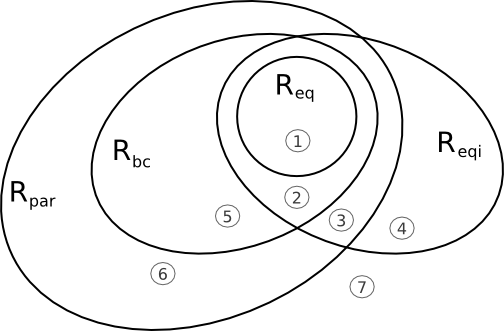
\includegraphics[width=300pt,height=241pt,keepaspectratio=true]
                    {containments.png}
  \end{center}
  \caption{ \label{fig:containments} Containment relationships for equivalence
    relations $R_{eq}$, $R_{eqi}$, $R_{bc}$, and $R_{par}$. The following are
    example elements in the sets at the specified locations: 1. (1100, 1100)
    2. (1010, 0101) 3. (1000, 0111) 4. (10000, 01111) 5. (1000, 0001) 6. (1000,
    1011) 7. (1000, 0000) }
\end{figure}


\section{Results}
\subsection{Reductions among equivalence relation}
\begin{theorem}$R_{par}\kr R_{bc}$\end{theorem}
\begin{proof}
\end{proof}
\begin{proof}
  Construct $M\in \FP$ on input $w\in\sigmastar$:
  \begin{algorithm}[h]
    \For{$i=1$ \KwTo $|w|-1$}{
      \If{$w_i=1$}{
        \For{$j=i+1$ \KwTo $|w|$}{
          \If{$w_j=1$}{
            write 0 to both $w_i$ and $w_j$\;
            break\;
          }
        }
      }
    }
  \end{algorithm}\\
  Notice that this is the machine which finds pairs of ones and writes zeros in
  their place, one pair at a time.

  Suppose $(x, y)\in R_{par}$, so either $x$ and $y$ both have even parity or
  $x$ and $y$ both have odd parity.
  
  If $x$ and $y$ both have even parity, $x$ contains $2k$ ones and $y$ contains
  $2l$ ones, for some $k,l\in\mathbb{N}$. $M(x)$ and $M(y)$ both output the
  string $0^{|x|}$, and since both $M(x)$ and $M(y)$ have a bitcount of zero,
  $(M(x), M(y))\in R_{bc}$.

  If $x$ and $y$ both have odd parity, $x$ contains $2k+1$ ones and $y$
  contains $2l+1$ ones, for some $k,l\in\mathbb{N}$. $M(x)$ and $M(y)$ both
  output a string containing a single one, so both $M(x)$ and $M(y)$ have a
  bitcount of one, $(M(x), M(y))\in R_{bc}$.

  Suppose $(x, y)\notin R_{par}$, so without loss of generality, $x$ has even
  parity and $y$ has odd parity. Then $x$ contains $2k$ ones and $y$ contains
  $2l+1$ ones, for some $k,l\in\mathbb{N}$. Thus $M(x)$ outputs the string
  $0^{|x|}$ and $M(y)$ outputs the string containing a single one. Since the
  bitcount of $M(x)$ is zero and the bitcount of $M(y)$ is one,
  $(M(x), M(y))\notin R_{bc}$.

  Therefore $(x, y)\in R_{par} \iff (M(x), M(y))\in R_{bc}$, so
  $R_{par} \kr R_{bc}$.
\end{proof}

\begin{theorem}$R_{bc}\kr R_{eq}$\end{theorem}
\begin{proof}
  Construct $M\in \FP$ on input $w\in\sigmastar$ which sorts the bits of $w$
  using an efficient (polynomial-time) sorting algorithm.

  Notice that if $|w|=n$ and $w$ contains $k$ ones, this machine outputs
  the string which can be described by the regular expression $0^{n-k}1^k$.

  Suppose $(x, y)\in R_{bc}$, so $x$ and $y$ have the same number of ones, say
  $k$. Thus $M(x)=M(y)=0^{n-k}1^k$, so $(M(x), M(y))\in R_{eq}$.
  
  Suppose $(x, y)\notin R_{bc}$, so $x$ and $y$ have a different number of
  ones. Suppose $x$ has $k$ ones and $y$ has $l$ ones, for some
  $k,l\in\mathbb{N}$. Assume without loss of generality that $k>l$. Then
  $M(x)=0^{n-k}1^{k}$ and $M(y)=0^{n-l}1^{l}$, so $M(x)\neq M(y)$. Thus
  $(M(x), M(y))\notin R_{eq}$.

  Therefore $(x, y)\in R_{bc} \iff (M(x), M(y))\in R_{eq}$, so $R_{bc}\kr
  R_{eq}$.
\end{proof}


\subsection{Reductions from equivalence relations to graph isomorphism}
\begin{theorem}\label{thm:rpar-gi}$R_{par}\kr GI$\end{theorem}
\begin{proof}
  Construct $M\in \FP$ on input $w\in\sigmastar$:\\
  \begin{algorithm}[H]
    $V_w\gets\{v_p, v_o\}$\;
    $E_w\gets\{\}$ \tcp{undirected edges}\;
    \For{$i=1$ \KwTo $|w|$}{
      \If{$w_i=1$}{
        \eIf{$(v_o, v_p)\in E_w$}{add undirected edge $(v_o, v_p)$ to $E_w$\;}
            {remove $(v_o, v_p)$ from $E_w$\;}
      }
    }
    \Return $G_w=(V_w, E_w)$
  \end{algorithm}

  Suppose $(x, y)\in R_{par}$, so either $x$ and $y$ both have even parity or
  $x$ and $y$ both have odd parity. 

  If $x$ and $y$ both have even parity, $x$ contains $2k$ ones and $y$ contains
  $2l$ ones, for some $k,l\in\mathbb{N}$. Since $2k$ is even, machine $M$ on
  input $x$ adds then removes the edge $(v_o, v_p)$ to and from $E_x$ an equal
  number of times. Similarly for $M$ on input $y$. Therefore $M(x)$ outputs
  $G_x=(V_x, E_x)$, where $V_x=\{v_o, v_p\}$ and $E_x=\{\}$, and $M(y)$ outputs
  $G_y=(V_y, E_y)$, where $V_y=\{v_o, v_p\}$ and $E_y=\{\}$. Then $G_x$ is
  isomorphic to $G_y$ by the identity function, $I:V_x\to V_y$, defined by
  $I(v)=v, \forall v\in V_x$.

  If $x$ and $y$ both have odd parity, $x$ contains $2k+1$ ones and $y$
  contains $2l+1$ ones, for some $k,l\in\mathbb{N}$. Since $2k+1$ is odd,
  machine $M$ on input $x$ adds edge $(v_o, v_p)$ to $E_x$ one more time than
  it removes the edge. Similarly for $M$ on input $y$. Therefore $M(x)$ outputs
  $G_x=(V_x, E_x)$, where $V_x=\{v_o, v_p\}$ and $E_x=\{(v_o, v_p)\}$, and
  $M(y)$ outputs $G_y=(V_y, E_y)$, where $V_y=\{v_o, v_p\}$ and $E_y=\{(v_o,
  v_p)\}$. Then $G_x$ is isomorphic to $G_y$ by the identity function,
  $I:V_x\to V_y$, defined by $I(v)=v, \forall v\in V_x$.

  Suppose $(x, y)\notin R_{par}$, so without loss of generality, $x$ has even
  parity and $y$ has odd parity. Then $x$ contains $2k$ ones and $y$ contains
  $2l+1$ ones, for some $k,l\in\mathbb{N}$. Since $2k$ is even, machine $M$ on
  input $x$ adds then removes the edge $(v_o, v_p)$ to and from $E_x$ an equal
  number of times. Since $2l+1$ is odd, machine $M$ on input $y$ adds edge
  $(v_o, v_p)$ to $E_y$ one more time than it removes the edge. Therefore
  $M(x)$ outputs $G_x=(V_x, E_x)$, where $V_x=\{v_o, v_p\}$ and $E_x=\{\}$, and
  $M(y)$ outputs $G_y=(V_y, E_y)$, where $V_y=\{v_o, v_p\}$ and $E_y=\{(v_o,
  v_p)\}$. Since $(v_o, v_p)\in E_y$ but $(v_o, v_p)\notin E_x$, so no
  bijection exists between $V_x$ and $V_y$ which preserves edges. Therefore,
  $G_x$ is not isomorphic to $G_y$.

  Therefore $(x, y)\in R_{par} \iff (M(x), M(y)) \in GI$, so $R_{par} \kr GI$.
\end{proof}

\begin{theorem}\label{thm:rbc-gi}$R_{bc}\kr GI$\end{theorem}
\begin{proof}
  Construct $M\in \FP$ on input $w \in \sigmastar$:\\
  \begin{algorithm}[H]
    $V_w\gets\{v_1, v_2, \ldots, v_{|w|}, v_{zero}, v_{one,0}, v_{one,1},
    v_{one,2}\}$\;
    $E_w\gets\{(v_{one,0}, v_{one,1}), (v_{one,1}, v_{one,2}), (v_{one,2},
    v_{one,0})\}$\tcp{undirected edges}\; 
    \For{$i=1$ \KwTo $|w|$}{
      \eIf{$w_i=1$}{
        add undirected edge $(v_i, v_{one,0})$ to $E_w$\;
      }{
        add undirected edge $(v_i, v_{zero})$ to $E_w$\;
      }
    }
    \Return{$G_w=(V_w, E_w)$}
  \end{algorithm}
  
  Suppose $(x, y)\in R_{bc}$, so $x$ and $y$ have the same number of ones, say
  $k\in\mathbb{N}$. Assume $|x|=|y|=n$, so both $x$ and $y$ have $n-k$
  zeros. Define $E_{w,1}=\{(v_i, v_{one,0})|i\in\{1,2,\ldots,n\}, w_i = 1\}$
  and $E_{w,0}=\{(v_i, v_{zero})|i\in\{1,2,\ldots,n\}, w_i = 0\}$, so $E_x =
  E_{x,1}\cup E_{x,0}$ and $E_y = E_{y,1} \cup E_{y,0}$ by construction. Define
  $V_{w,b}=\{v_i|w_i=b\}$, so $V_x=V_{x,1} \cup V_{x,0}$ and $V_y=V_{y,1} \cup
  V_{y,0}$. Note that $|V_{x,1}|=|V_{y,1}|=k$ and
  $|V_{x,0}|=|V_{y,0}|=n-k$. Since $|V_{x,1}|=|V_{y,1}|=k$, there exists a
  bijection between them, call it $\phi_1:V_{x,1}\to V_{y,1}$. Similarly, since
  $|V_{x,0}|=|V_{y,0}|=k$, there exists a bijection between them, call it
  $\phi_0:V_{x,0}\to V_{y,0}$. Define $\phi:V_x\to V_y$ by
  \begin{displaymath}
    \phi(v) = 
    \begin{cases}
      \phi_0(v) & \plain{if} v = v_i \plain{and} x_i = 1, \plain{for some}
      i\in\{1,\ldots,n\}\\ 
      \phi_1(v) & \plain{if} v = v_i \plain{and} x_i = 0, \plain{for some}
      i\in\{1,\ldots,n\}\\ 
      v & \plain{if} v \in \{v_{zero}, v_{one,0}, v_{one,1}, v_{one,2}\}
    \end{cases}
  \end{displaymath}
  for all $v\in V_x$. Notice that each $v_i$ ``corresponds'' to a
  single $x_i$, because each $x_i$ can be either a one or a zero,
  exclusively.

  Since the only edges in $E_x$ are the edges $(v_i, v_{one,0})$ when $x_i=1$
  and $(v_i, v_{zero})$ when $x_i=0$, then $(v_i, v_{one,0})\in E_x \iff
  (\phi(v_i), \phi(v_{one,0}))=(\phi_1(v_i), v_{one,0})\in E_y$, and $(v_i,
  v_{zero})\in E_x \iff (\phi(v_i), \phi(v_{zero})) = (\phi_0(v_i),
  v_{zero})\in E_y$. Therefore $\phi$ describes a graph isomorphism, so $G_1$
  is isomorphic to $G_2$.
  
  Suppose $(x, y)\notin R_{bc}$, so $x$ and $y$ have a different number of
  ones. Let $k$ be the number of ones in $x$, and $l$ be the number of ones in
  $y$, with $k\neq l$. Suppose without loss of generality that $k>l$. Define
  $E_{w,0}$ and $E_{w,1}$ as above. Now $|E_{x,1}|=k$ and $|E_{y,1}|=l$. Since
  $k>l$, $E_{x,1}$ has at least one more edge adjacent to the triangle created
  by the vertices $\{v_{one,0},v_{one,1},v_{one,2}\}$ than does $E_{y,1}$. Thus
  no possible bijection exists between $V_x$ and $V_y$ which preserves all
  edges. Thus $G_x$ is not isomorphic to $G_y$, so $(M(x), M(y))\notin GI$.

  Therefore $(x, y)\in R_{bc} \iff (M(x), M(y))\in GI$, so $R_{bc}\kr GI$.
\end{proof}

\begin{theorem}\label{thm:req_kr_gi}$R_{eq} \kr GI$\end{theorem}
\begin{proof}
  Construct machine $M\in\FP$ on input $w\in\sigmastar$:
  \begin{enumerate}
  \item Initialize set of vertices $V_w=\{v_1, v_2, \ldots, v_{|w|}\}$
    and set of directed edges $E_w=\{(v_1, v_2),(v_2,
    v_3),\ldots,(v_{|w|-1}, v_{|w|})\}$.
  \item For $i=1$ to $|w|$:
    \begin{enumerate}
    \item If $w_i=1$, add vertex $v'_i$ to $V_w$ and directed edge $(v_i,
      v'_i)$ to $E_w$.
    \end{enumerate}
  \item Output $G_w=(V_w, E_w)$.
  \end{enumerate}
  This machine constructs a ``spine'' of vertices, with an extra vertex $v'_i$
  and directed edge $(v_i, v'_i)$ adjacent to the spine whenever $w_i$ is a
  one, $\forall i\in\{1,2,\ldots,|w|\}$.

  Suppose $(x, y)\in R_{eq}$, so $x=y$. Then $M(x)$ and $M(y)$ obviously
  produce the same graph, so $(M(x), M(y))\in GI$.
  
  %% TODO is this sufficient proof?

  Suppose $(x, y)\notin R_{eq}$, so $x\neq y$. Suppose $|x|=|y|=n$. Run $M$ on
  input $x$ to yield $G_x=(V_x, E_x)$, and run $M$ on input $y$ to yield
  $G_y=(V_y, E_y)$. Since the graphs are directed, the ``spine'' created by the
  vertices $\{v_1, v_2, \ldots, v_n\}$ and the edges $\{(v_1, v_2), (v_2, v_3),
  \ldots, (v_{n-1}, v_n)\}$ must correspond in both $G_x$ and $G_y$. Let $i$ be
  the index of the first bit at which $x$ and $y$ differ. Suppose without loss
  of generality that $x_i=1$ and $y_i=0$. Then $v'_i\in V_x$ and $(v_i,
  v'_i)\in E_x$, but $v'_i\notin V_y$ so $(v_i, v'_i)\notin E_y$. Since
  vertices along the ``spine'' of the $V_x$ must map to vertices along the
  ``spine'' of $V_y$, and specifically $v_i$ in $V_x$ must map to $v_i$ in
  $V_y$, $(v_i, v'_i)\in E_x$ implies $(v_i, v'_i)\in E_y$. But no such mapping
  can exist, because $(v_i, v'_i)\notin E_y$. Therefore $G_x$ is not isomorphic
  to $G_y$, so $(M(x), M(y))\notin GI$.

  Therefore $(x, y)\in R_{eq} \iff (M(x), M(y))\in GI$, so $R_{eq}\kr GI$.  
\end{proof}

\begin{theorem}$R_{eqi}\kr GI$\end{theorem}
\begin{proof}
  Construct machine $M\in \FP$ on input $w\in\sigmastar$:
  \begin{enumerate}
  \item Initialize set of vertices $V_w=\{v_{zero}, v_{one}, v_1, v_2, \ldots,
    v_{|w|}\}$ and set of directed edges $E_w=\{(v_1, v_2), (v_2, v_3), \ldots,
    (v_{|w|-1}, v_{|w|})\}$.
  \item For $i=1$ to $|w|$:
    \begin{enumerate}
    \item If $w_i=1$ add directed edge $(v_i, v_{one})$ to $E_w$.
    \item If $w_i=0$ add directed edge $(v_i, v_{zero})$ to $E_w$.
    \end{enumerate}
  \item Output $G_w=(V_w, E_w)$.
  \end{enumerate}
  Notice that this machine, as in the machine in the proof of Theorem
  \ref{thm:req_kr_gi}, creates a ``spine'' representing each bit of word
  $w$.

  Suppose $(x, y)\in R_{eqi}$, so either $x=y$ or $x=\bar{y}$.

  If $x=y$, $M(x)$ and $M(y)$ output exactly the same graph, so $G_x$ is
  isomorphic to $G_y$, and hence $(M(x), M(y))\in GI$.

  If $x=\bar{y}$, define $\phi:V_x\to V_y$ by
  \begin{displaymath}
    \phi(v)=
    \begin{cases}
      v & \plain{if} v = v_i\\
      v_{zero} & \plain{if} v = v_{one}\\
      v_{one} & \plain{if} v = v_{zero}
    \end{cases}
  \end{displaymath}
  for all $v\in V_x$. Notice that $\phi$ maps each $v_i\in V_x$ to the
  corresponding $v_i\in V_y$, and maps $v_{zero}\in V_x$ to $v_{one}\in V_y$
  and $v_{one}\in V_x$ to $v_{zero}\in V_y$. Then $\forall
  i\in\{1,2,\ldots,|x|\}$, $x_i=0 \iff y=1$, so $(v_i, v_{zero})\in E_x \iff
  (\phi(v_i), \phi(v_{zero}))\in E_y \iff (v_i, v_{one})\in E_y$. Similarly,
  $x_i=1 \iff y=0$, so $(v_i, v_{one})\in E_x \iff (\phi(v_i),
  \phi(v_{one}))\in E_y \iff (v_i, v_{zero})\in E_y$. The rest of the edges in
  $E_x$ map directly to the corresponding edges in $E_y$ by $(v_{i-1}, v_i)
  \mapsto (\phi(v_{i-1}), \phi(v_i))=(v_{i-1}, v_i)$, $\forall
  i\in\{2,3,\ldots,|x|\}$. Therefore, $\phi$ describes an isomorphism between
  $G_x$ and $G_y$, so $(M(x), M(y))\in GI$.

  Suppose $(x, y)\notin R_{eqi}$, so $x\neq y$ and $x\neq\bar{y}$. Thus
  $\exists i,j\in\{1,2,\ldots,|x|\}, i\neq j,$ such that $x_i=y_i\land x_j\neq
  y_j$. Suppose without loss of generality that $x_i=y_i=0$ and $0=x_j\neq
  y_j=1$. Now $x_i=y_i=0$ implies $(v_i, v_{zero})\in E_x$ and $(v_i,
  v_{zero})\in E_y$. Also, $x_j=0$ implies $(v_j, v_{zero})\in E_x$ and $y_j=1$
  implies $(v_j, v_{one})\in E_y$. Assume, with the goal of producing a
  contradiction, that there exists a bijection, $\phi:V_x\to V_y$ such that
  $(u,v)\in E_x\iff(\phi(u),\phi(v))\in E_y$. Since $\phi$ must map vertices
  on the ``spine'' of $G_x$ to corresponding vertices in $G_y$, and since
  $(v_i, v_{zero})\in E_x$, then $(\phi(v_i), \phi(v_{zero}))=(v_i,
  \phi(v_{zero}))$ must be in $E_y$. The only edge of this form in $E_y$ is
  $(v_i, v_{zero})$ so $\phi(v_{zero})=v_{zero}$. Since $(v_j, v_{zero})\in
  E_x$, $(\phi(v_j), \phi(v_{zero}))=(v_j, v_{zero})\in E_y$. But the only edge
  in $E_y$ with source vertex $v_j$ is, by construction, $(v_j, v_{one})$. This
  is a contradiction. Hence no such bijection exists, so $G_x$ is not
  isomorphic to $G_y$, and $(M(x), M(y))\notin GI$.

  Therefore $(x, y)\in R_{eqi} \iff (M(x), M(y))\in GI$, so $R_{eqi}\kr GI$.
\end{proof}


\subsection{Completeness}
\begin{theorem}\label{thm:krc_npc}If a language $A$ is $\kr$-complete in \NPEq,
  then $A$ is $\mor$-complete in \NP. In other words, if $A$ is \NPEq-complete
  then $A$ is \NP-complete.\end{theorem}
\begin{proof}
  %% TODO complete this proof
\end{proof}

\begin{corollary}\label{cor:gi_complete}If $GI$ is not $\mor$-complete in
	\NP\,then $GI$ is not $\kr$-complete in \NPEq. In other words, if $GI$ is not
  \NP-complete then $GI$ is not \NPEq-complete.\end{corollary}
\begin{proof}
  This is a specific case of the contrapositive statement of Theorem
  \ref{thm:krc_npc}.
\end{proof}

\begin{definition}\label{def:gim_class}$\GIm$ is the class of problems which
  are polynomial-time, many-one equivalent to $GI$. In other words,
  $\GIm=\{A|A\moequiv GI\}$.\end{definition}

\begin{definition}\label{def:giker_class}$\GIker$ is the class of problems
	which are polynomial-time equivalent under kernel reductions to $GI$. In
	other words, $\GIker=\{A|A\kequiv GI\}$.\end{definition}

\begin{theorem}If $GI$ is not \NP-complete then $\NPEq\neq\GIker$. In other
	words, there exists a language $B$ in \NPEq\,such that $B\nkr
	GI$.\end{theorem}
\begin{proof}
	Suppose $GI$ is not \NP-complete. By Corollary \ref{cor:gi_complete}, $GI$ is
  not \NPEq-complete. Assume $\GIker=\NPEq$. By Definition
  \ref{def:giker_class}, $GI$ is complete under kernel reductions in
  $\GIker$. Hence $GI$ is complete under kernel reductions in \NPEq, or in
  other words, $GI$ is \NPEq-complete. This is a contradiction. Therefore
  $\GIker\neq\NPEq$.

  %% TODO complete this proof
\end{proof}


\section{References}
%\bibliography{references}

\end{document}
